\documentclass{article}
\usepackage[T1]{fontenc}
\usepackage{lmodern}
\usepackage{graphicx}
\usepackage{amsmath,amssymb}
\usepackage[a4paper,margin=2cm]{geometry}
\usepackage[absolute,overlay]{textpos}
\setlength{\TPHorizModule}{1mm}
\setlength{\TPVertModule}{1mm}
\usepackage[indonesian]{babel}
\usepackage{hyperref}
\setlength{\emergencystretch}{2em}
% unit: Halaman 2

\begin{document}

% === Halaman 2 (python/native) ===

• Misalkan Alice dan Bob saling berkomunikasi dengan berkirim pesan:


- via surat menyurat,


- via telepon


- via email


- via SMS


- dll

menggunakan saluran komunikasi publik (pos, telepon, jaringan seluler, internet)

2

% deskripsi: gambar native xref 25
\noindent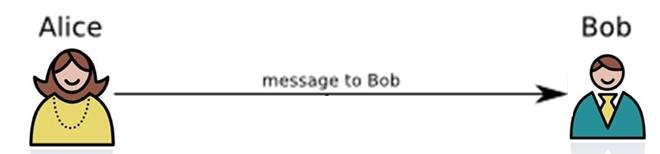
\includegraphics[width=0.85\textwidth]{../../images/python/page_002_img_01.jpeg}

\end{document}
